\begin{frame}{One pipeline, two deliberately separated tracks}
\begin{center}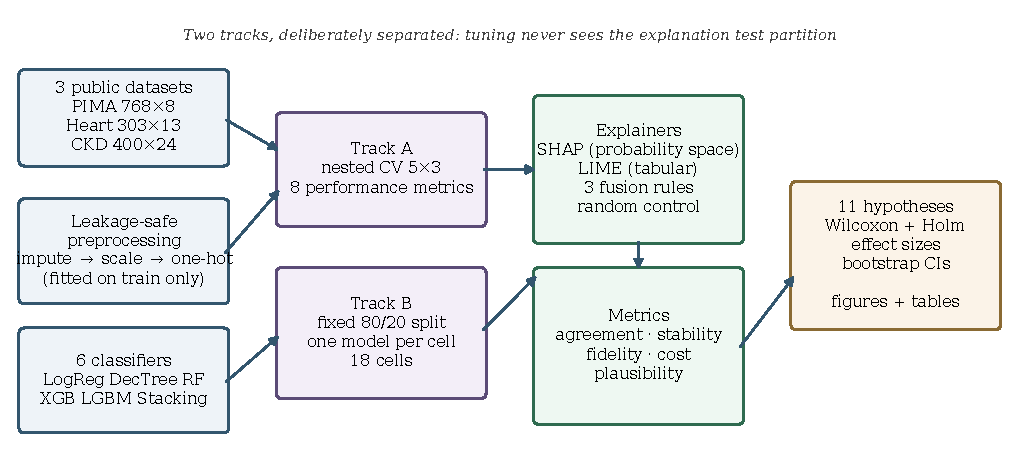
\includegraphics[width=0.95\textwidth]{F1.pdf}\end{center}
\takeaway{Track A tunes and scores. Track B explains a model whose test partition never
took part in tuning. Conflating them is how explanation studies leak.}
\end{frame}

\begin{frame}{Three datasets chosen to span a difficulty gradient}
\begin{columns}[T]
\begin{column}{0.5\textwidth}
\small
\begin{tabular}{@{}lrrr@{}}
\toprule
Dataset & $n$ & Feat. & ROC-AUC \\
\midrule
PIMA Diabetes & 768 & 8 & \AucPima{} \\
Heart Disease & 303 & 13 & \AucHeart{} \\
Chronic Kidney & 400 & 24 & \AucCkd{} \\
\bottomrule
\end{tabular}
\medskip
\footnotesize All public, de-identified, redistributable.\\
Diseases are \textbf{benchmarks}. No medical claims.
\end{column}
\begin{column}{0.5\textwidth}
\begin{itemize}\setlength\itemsep{0.4em}
  \item 6 classifiers: LogReg, DecTree, RF, XGBoost, LightGBM, Stacking
  \item 6 explainers: \shap{}, \lime{}, 3 fusion rules, \textbf{random control}
  \item 16 interpretability measures across 5 families
\end{itemize}
\end{column}
\end{columns}
\takeaway{A single dataset cannot ask whether explainer agreement depends on how hard
the decision boundary is. Three, spanning \AucPima{} to \AucCkd{}, can.}
\end{frame}

\begin{frame}{Four traps that silently invalidate this comparison}
\small
\begin{enumerate}\setlength\itemsep{0.55em}
  \item \textbf{Different output spaces.} \lime{} explains probability; tree \shap{}
    defaults to log-odds. We force probability space and \emph{verify} it by additivity
    --- median error \AdditivityMedianMax{}.
  \item \textbf{Synthetic reference points.} A $k$-means background averages one-hot
    columns into values the model never sees. That broke \shap{}'s own additivity by
    $9.9\times10^{-3}$ on LightGBM. Fixed: real training rows.
  \item \textbf{One-hot fragmentation.} Deleting ``the top 5 features'' must delete all
    their columns --- otherwise a 25-column dataset is under-perturbed and an 8-column
    one is not.
  \item \textbf{No control, no scale.} Deleting any few features moves a prediction, so
    \aopc{} $=0.31$ means nothing alone. Every number is reported against a random
    ranking.
\end{enumerate}
\takeaway{None of these is visible in the output when it goes wrong. Three were caught
by tests we wrote before running.}
\end{frame}
